\RequirePackage{luatex85}
\documentclass[%
 % reprint,
% superscriptaddress,
% groupedaddress,
% unsortedaddress,
% runinaddress,
% frontmatterverbose,
% preprint,
% preprintnumbers,
% nofootinbib,
% nobibnotes,
% bibnotes,
 amsmath,amssymb,
aps,
% pra,
% prb,
% rmp,
% prstab,
% prstper,
% floatfix,
 fleqn,
 notitlepage,
]{revtex4-2}

\usepackage{graphicx}% Include figure files
\usepackage{dcolumn}% Align table columns on decimal point
\usepackage{bm}% bold math
\usepackage{hyperref}% add hypertext capabilities
\usepackage{xcolor}
\usepackage{unicode-math}
\usepackage{fancyref}
\usepackage{siunitx}
\usepackage{soul}
\usepackage{nccmath}
\usepackage{tikz}
\usepackage{subcaption}
\usepackage{float}
% \endofdump

\usetikzlibrary{calc, patterns, decorations.pathmorphing, decorations.markings}
\tikzset{
    ground/.style = {
        fill,
        pattern        = north east lines,
        draw           = none,
        minimum width  = 0.5cm,
        minimum height = 0.3cm,
    },
}

%\usepackage[mathlines]{lineno}% Enable numbering of text and display math
%\linenumbers\relax % Commence numbering lines

%\usepackage[showframe,%Uncomment any one of the following lines to test
%%scale=0.7, marginratio={1:1, 2:3}, ignoreall,% default settings
%%text={7in,10in},centering,
%%margin=1.5in,
%%total={6.5in,8.75in}, top=1.2in, left=0.9in, includefoot,
%%height=10in,a5paper,hmargin={3cm,0.8in},
%]{geometry}

\usepackage[
    margin=1.2in,
    a4paper
]{geometry}

\expandafter\hypersetup{
  pdftitle = {Grungy Times: The Euler-Lagrange Equations},
  pdfauthor = {Anshul Singhvi},
  pdfdisplaydoctitle = true,
  colorlinks,
  linkcolor={red!50!black},
  citecolor={blue!50!black},
  urlcolor={blue!80!black}
}

% \onehalfspacing


\begin{document}

\preprint{APS/123-QED}

\title{Grungy Times: The Euler-Lagrange Equations}

\author{Anshul Singhvi}
\altaffiliation[Also at ]{Applied Physics Department, Columbia University.}
\email{asinghvi17@simons-rock.edu}
\author{Bethan Cordone}
\altaffiliation[Also at ]{Applied Physics Department, Columbia University.}
\email{bcordone17@simons-rock.edu}
\author{Prutha Patil}%
\email{ppatil18@simons-rock.edu}
\author{Yecheng Ma}
\altaffiliation[Also at ]{Operations Research Department, Columbia University.}
\email{yma17@simons-rock.edu}
\author{YuXuan Liu}
\altaffiliation[Also at ]{Applied Physics Department, Columbia University.}
\email{yliu17@simons-rock.edu}

\affiliation{Bard College at Simon's Rock}%

\date{\today}% It is always \today, today,
             %  but any date may be explicitly specified

\maketitle

\linespread{1.3}

\section{Introduction}
% https://www.youtube.com/watch?v=oHg5SJYRHA0, here's something fun for everyone.
% Euler-Lagrange forms an integral part of our petrochemical production pipeline.

For systems with one degree of freedom, the \emph{action integral}, called $J(y)$, can be expressed as:

\begin{equation}\label{eq: action}
    J(y) = \int_a^b F(x, y, \dot y) ~ dx
\end{equation}

To solve for the equations of motion of a mechanical system, we can attempt to find function $y(t)$ which is a \emph{stationary point} of the action integral; this means that the trajectory which $y(t)$ takes conserves the quantity within the action integral.  This function must satisfy several constraints; it must satisfy the boundary conditions $y(a) = A$, and $y(b) = B$, and it must have at least two continuous derivatives.

It's useful to examine the behaviour around our proposed solution, to see whether it really is a stationary point.  This method is known as the \textit{calculus of variations}.
Consider a perturbation to the initial function, of magnitude $0 < \epsilon \ll 1$:

\[
    \bar y(t) = y(t) + \epsilon \cdot \eta(t)
\]

$\eta(t)$ is called the \textit{perturbation function}; it is simply a function which obeys $\eta(a) = 0$ and $eta(b)$ = 0.  Now, we can observe the behaviour of the action integral as a function of $\epsilon$:

\[
    \phi(\epsilon) = J(y + \epsilon \cdot \eta) = \int_a^b F(x, y + \epsilon \eta, \dot y + \epsilon \dot \eta) ~ dx
\]

We can evaluate the \emph{derivative} of $\phi$ at 0.  We know, however, that there must be a stationary point at $\epsilon = 0$, which leads us to the inevitable conclusion that we must relinquish ourselves to the greedy clutches of algebra, and evaluate $\frac{d\phi}{d\epsilon}=0$ at $\epsilon=0$.

After some simplification, this evaluation becomes:
\[
    \int_{a}^{b}\left[\frac{\partial F}{\partial y}\left(x, \bar{y}, \bar{y}^{\prime}\right)-\frac{\partial^{2} F}{\partial x \partial y^{\prime}}\left(x, \bar{y}, \bar{y}^{\prime}\right)\right] \eta ~ d x=0
\]

which means that the multiplicand of $\eta$ must be 0.  Therefore,

\[
    \frac{\partial F}{\partial y}\left(x, y, y^{\prime}\right)-\frac{\partial^{2} F}{\partial x \partial y^{\prime}}\left(x, y, y^{\prime}\right)=0
\]

which is the Euler-Lagrange equation.


For our mechanical systems, the value being integrated in $J(y)$ is the kinetic energy minus the potential energy: $K-V$. In the physical sciences, this is known as the Lagrangian, and is usually denoted by $\mathscr L$.

Thus, the solution to the action integral is the Euler-Lagrange equation:

\begin{equation}\label{eq: el}
    \frac{∂}{∂y} \left[\vphantom{\frac12} \mathscr L(t, y, \dot y) \right] - \frac{∂^2}{∂x∂\dot y} \left[\vphantom{\frac12} \mathscr L(x, y, \dot y) \right] = 0
\end{equation}

\section{Falling Bodies} % q1

Any body falling sufficiently close to the surface of the Earth is subject to an approximately constant gravitational force $F = mg$, assuming a perfectly spherical Earth, and that the object's height above the surface of the Earth is much less than its radius.  Its trajectory is parameterized by a function $y(t)$ which expresses its height relative to the surface of the Earth.  We concern ourselves here with a trajectory going from $t = 0, y_0 = y(0)$ to $t = T, y = y(T)$.

The kinetic energy of a falling body is simply $\displaystyle T = \frac12 m\dot y^2$.  Its gravitational potential energy is the integral of the gravitational force from its origin to its destination; assuming the surface of the Earth as the origin ($y = 0$), $\displaystyle V = mgy$.

We have defined an isolated system; as such, in the confines of the system, there can be no change in the net amount of energy.  The energy can be represented $E_{tot} = T - V$, which expands to $\displaystyle E_{tot} = \frac12m\dot y(t)^2 - mgy(t)$.  This function $E_{tot}(t, y, \dot y)$ is what we need to conserve.

Thus, we can define the action integral $J$ as follows:
\[
    J = \int_0^T \frac12m\dot y(t)^2 - mgy(t) ~ dt
\]

By the Euler-Lagrange constraint, then,

\begin{align*}
  &\frac{∂}{∂y} \left[E_{tot}(t, y, \dot y)\right] - \frac{∂^2}{∂t∂y} \left[E_{tot}(t, y, \dot y)\right] = 0
\end{align*}

We can evaluate these partial derivatives, of course, and this evaluation gives us the equation:

\begin{align*}
  &m\ddot y(t) = -mg\\
  &⟹ \ddot y(t) = -g\\
\end{align*}

This can now be integrated with respect to time.

\begin{align*}
  &\iint \ddot y(t) ~ dt ~ dt = \iint -g ~ dt ~ dt\\
  &⟹ y(t) = \iint -g ~ dt ~ dt\\
  &⟹ y(t) = \int -gt + C_1 ~ dt\\
  &⟹ y(t) = -\frac12gt^2 + C_1t + C_2\\
\end{align*}

The constants $C_1$ and $C_2$ are really just the initial velocity and position of the object, respectively.  This function describes a parabolic trajectory, which we know to be true.

\section{The Brachistochrone Problem} % q3

The brachistochrone curve is simply the curve along which a frictionless particle will slide in the minimum time. Brachistochrone trajectories are especially interesting in the context of space travel, since they provide the most efficient trajectories with which to traverse long distances. It also has applications in our everyday lives; for example, creating efficient roller coasters, or

The problem is, specifically, to find the curve $y(x)$ between points $y(a) = A$ and $y(b) = B$, along which a particle will slide in the minimum time. We need to find a balance between the speed of the particle and the length of the path.

Here, we will trace out Johann Bernoulli's solution to the brachistochrone problem, and justify all the steps he took.

We begin with the fundamental theorem of calculus, which shows that:
\[T = \int_0^t dt\]

Next, we proceed to a chain rule equality.  Though this is perhaps unpalatable to most mathematicians, it is trivial to show through the chain rule that $\frac{dt}{ds} ds = dt$:

\[\implies \int_0^T dt = \int_0^L \frac{dt}{ds} ds\]

However, there is an important simplification we can make here.  Velocity is defined as $v = \frac{ds}{dt}$, and a simple inversion shows that $\frac{dt}{ds} = \frac 1v$:

\[\int_0^L \frac{dt}{ds} ds = \int_0^L \frac 1v ~ ds\]

Let us assume a coordinate system in which the particle begins at the origin, and the positive $y$ direction points upwards, against the direction of gravity.  We can now find the velocity of the particle as a function of its position, by using the principle of energy conservation.

Additionally, let $h = 0$ be the initial position of the particle.  We know that the gravitational potential energy is simply $V_g = mgh$, and that the kinetic energy in the absence of rotation or friction is $T = \frac12 mv^2$.  Thus,

\begin{align*}
    &mgh = -mgy + \frac12 mv^2\\
    &\implies mgy = \frac12 mv^2\\
    &\implies v = \sqrt{2gy}
\end{align*}

Now, we can substitute this back into our original integral,

\[\int_0^L \frac 1v ~ ds = \int_0^L \frac{1}{\sqrt{2gy}} ~ ds\]

However, it's important to remember that here, $ds$ is actually just $\sqrt{dx^2 + dy^2}$.  This can then be algebraically simplified to $dx\sqrt{1 - \left(\frac{dy}{dx}\right)^2}$.  Substituting this into our integral,

\[\int_0^L \frac{1}{\sqrt{2gy}} ~ ds = \sqrt{\frac{1}{2g}} \int_a^b \sqrt{\frac{1 + y'^2}{y}} ~ dx\]

This is simply integrating over the $x$ domain of the path, as opposed to the $y$ domain.

We can now solve for the Euler-Lagrange equations of $\displaystyle \sqrt{\frac{1}{2g}} \int_a^b \sqrt{\frac{1 + y'^2}{y}} ~ dx$:

\begin{align*}
    &F_{y}=-\sqrt{\frac{1+(y')^2}{8 g}} y^{-\frac32}\\
    &F_{y^{\prime}}=\frac{y}{\sqrt{2 g y} \sqrt{1+(y')^2}}\\
    &F_{y^{\prime} x}=\frac{\frac{1}{2} y^{\prime 2}\left[y\left(1+y^{\prime 2}\right)\right]^{-1 / 2}\left(2 y^{\prime \prime} y+y^{\prime 2}+1\right)+y^{\prime \prime}(\sqrt{y} \sqrt{1+y^{\prime 2}})}{\sqrt{2 g y\left(1+y^{\prime 2}\right)}}
\end{align*}

We know that $F_{y'x} = F_y$.  Therefore, % TODO justify

\begin{align*}
    &\sqrt{\frac{1+y^{\prime 2}}{8 g}} y^{-\frac{3}{2}}-\frac{\frac{1}{2} y^{\prime 2}\left[y\left(1+y^{\prime 2}\right)\right]^{-1 / 2}\left(2 y^{\prime \prime} y+y^{\prime 2}+1\right)+y^{\prime \prime}(\sqrt{y} \sqrt{1+y^{\prime 2}})}{\sqrt{2 g y\left(1+y^{\prime 2}\right)}}=0\\
    &\text{After some tedious simplification, which is redacted for clarity,}\\
    &2y''y' + y'^2 + 1 = 0 & \Box
\end{align*}

\begin{figure}[ht!]
    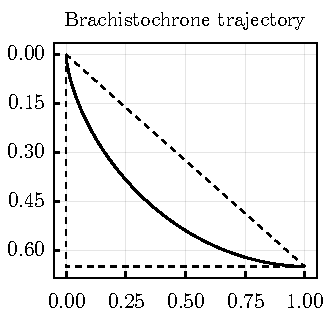
\includegraphics{brachistochrone.pdf}
    \caption{The brachistochrone trajectory from (0, 0) to (1, -0.65).  The dashed lines represent linear, slower paths.}
    \label{fig: brachistochrone}
\end{figure}

This can be shown to be the equation of a cycloid, and \Fref{fig: brachistochrone} illustrates one such trajectory.

\section{The Spring-Mass System} % q2


Spring-mass systems are very common in physics.  Let us define a system with a single mass, tethered to a wall by a spring.  Let it have a degree of freedom along the $x$-axis, and let the origin be at the equilibrium point.  Amen.

\begin{figure}[h!]
    \centering
    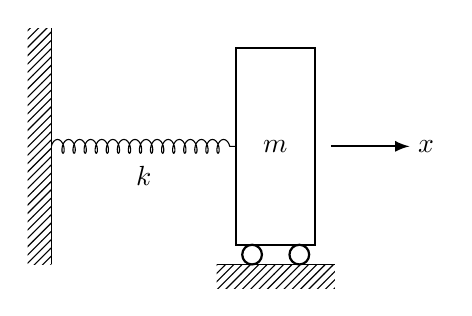
\begin{tikzpicture}[every node/.style = {draw, outer sep = 0pt, thick}]
        \node (M) [minimum width=1cm, minimum height=2.5cm] {$m$};

        \node (ground) [ground,anchor=north,yshift=-0.25cm,minimum width=1.5cm] at (M.south) {};
        \draw (ground.north east) -- (ground.north west);
        \draw [thick] (M.south west) ++ (0.2cm, -0.125cm) circle (0.125cm)  (M.south east) ++ (-0.2cm, -0.125cm) circle (0.125cm);

        \node (wall) [ground, rotate=-90, minimum width=3cm,yshift=-3cm] {};
        \draw (wall.north east) -- (wall.north west);

        \draw [decorate, decoration = {coil, segment length=4pt}] (wall.east) ++ (0.15cm, 1.5cm) -- (M.west) node [midway, below = 4pt, draw = none] {$k$};

        \draw [-latex, thick] (M.east) ++ (0.2cm, 0) -- +(1cm, 0) node [right, draw = none,] {$x$};

    \end{tikzpicture}
    \caption{A single-spring, single-mass system.}
\end{figure}

The elastic potential energy in this system is simply $\displaystyle V(x) = \frac12kx^2$, where $k$ is the constant of compressibility of the spring.  The formula for kinetic energy is unchanged ($\displaystyle T(\dot x) = \frac12m\dot x^2$).  Knowing these, the conserved term is $\displaystyle \mathscr L = T - V = \frac12m\dot x^2 - \frac12kx^2$.

From this, we can directly solve for the Euler-Lagrange equations:
\begin{align*}
  &\frac{∂\mathscr L}{∂x} = -kx\\
  &\frac{∂\mathscr L}{∂t∂x} = m\ddot x\\
  &⟹ m\ddot x + kx = 0\\
\end{align*}

This last expression is the differential equation which governs spring motion.

\section{Generalising the Lagrangian: Degrees of Freedom} % q6

Until now, we have only considered systems with one degree of freedom (position).  However, the Euler-Lagrange method is powerful!  We can easily generalize it to an arbitrary number of degrees of freedom.  Here, we will consider the case of a system with two degrees of freedom - represented by two coordinates, $x$ and $y$.


Such a system would form an action integral of:
\[
    J(x, y)=\int_{a}^{b} F\left(t, x, y, x^{\prime}, y^{\prime}\right) ~ dt
\]
The perturbed functional would then be:

\begin{align*}
\phi(\epsilon) &=J(\bar{x}+\epsilon n_x, \bar{y}+\epsilon n_y) \\
&=\int_{a}^{b} F\left(t, \bar{x}+\epsilon n_x, \bar{y}+\epsilon n_y, \bar{x}^{\prime}+\epsilon n_x^{\prime}, \bar{y}^{\prime}+\epsilon n_y^{\prime}\right) d t
\end{align*}

where $\langle n_x(t),n_y(t)\rangle$ is a small vector perturbations to the system that satisfies:
\[
    \left\langle n_x(a),n_y(a)\right\rangle = \left\langle 0,0 \right\rangle \qquad \left\langle n_x(b),n_y(b) \right\rangle = \left\langle 0,0 \right\rangle
\]

Differentiating the perturbed functional $\phi(\epsilon)$, with respect to $\epsilon$,

\[
    \frac{d\phi}{d\epsilon} = \left.\frac{d J(t,x+\epsilon n_x, y+\epsilon n_y,x'+\epsilon n'_x,y'+\epsilon n'_y)}{d\epsilon}\right|_{\epsilon=0}
\]

We can derive this to be:

\begin{align*}
    &= \int_a^b \left(\frac{\partial F}{\partial x}n_x + \frac{\partial F}{\partial x'}n_x' + \frac{\partial F}{\partial y}n_y + \frac{\partial F}{\partial y'}n_y'\right)dt\\
    &= \int_a^b \left(\frac{\partial F}{\partial x}n_x + \frac{\partial F}{\partial x'}\frac{d n_x}{dt} + \frac{\partial F}{\partial y}n_y + \frac{\partial F}{\partial y'}\frac{d n_y}{dt}\right)dt\\
    &= \left.\left(\frac{\partial F}{\partial x'}n_x(t) + \frac{\partial F}{\partial y'}n_y(t)\right)\right|_{t=a}^b + \int_a^b \left(\frac{\partial F}{\partial x}n_x - n_x\frac{d}{dt}\frac{\partial F}{\partial x'} + \frac{\partial F}{\partial y}n_y - n_y\frac{d}{dt}\frac{\partial F}{\partial y'}\right)dt\\
    &\text{The boundary terms can be set to zero, from the constraint on pertubation vectors:}\\
    &= \int_a^b \left(\frac{\partial F}{\partial x}n_x - n_x\frac{d}{dt}\frac{\partial F}{\partial x'} + \frac{\partial F}{\partial y}n_y - n_y\frac{d}{dt}\frac{\partial F}{\partial y'}\right)dt\\
    &= \int_a^b \left(\left[\frac{\partial F}{\partial x} - \frac{d}{dt}\frac{\partial F}{\partial x'}\right]n_x + \left[\frac{\partial F}{\partial y} - \frac{d}{dt}\frac{\partial F}{\partial y'}\right]n_y\right)dt = 0\\
\end{align*}

Since this condition must hold for any choice of $n_x,n_y$, it is sufficient to conclude that the integrand itself must be zero, i.e. that each multiple of $n_x,n_y$ must be zero.

This relationship can be summarized as a pair of Lagrange equations:
\[\frac{\partial F}{\partial x} - \frac{d}{d t}\frac{\partial F}{\partial x'}=0\]
\[\frac{\partial F}{\partial y} - \frac{d}{d t}\frac{\partial F}{\partial y'}=0\]

\section{The Two Mass, Three Spring System} % q4


\begin{figure}[H]
    \centering
    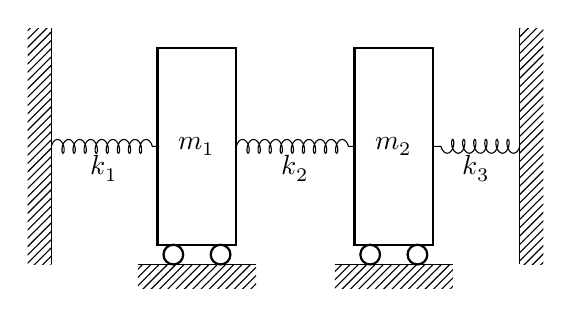
\begin{tikzpicture}[every node/.style = {draw, outer sep = 0pt, thick}]
        \node at (0, 0) (M) [minimum width=1cm, minimum height=2.5cm] {$m_1$};

        \node (ground) [ground,anchor=north,yshift=-0.25cm,minimum width=1.5cm] at (M.south) {};
        \draw (ground.north east) -- (ground.north west);
        \draw [thick] (M.south west) ++ (0.2cm,-0.125cm) circle (0.125cm)  (M.south east) ++ (-0.2cm,-0.125cm) circle (0.125cm);

        \node (wall) [ground, rotate=-90, minimum width=3cm, yshift=-2cm] {};
        \draw (wall.north east) -- (wall.north west);

        \draw [decorate, decoration = {coil, segment length=4pt}] (wall.east) ++ (0.15cm, 1.5cm) -- (M.west) node [midway, below, draw = none] {$k_1$};

        \node at (2.5, 0) (M2) [minimum width = 1cm, minimum height = 2.5cm] {$m_2$};
        \node (ground) [ground,anchor=north,yshift=-0.25cm,minimum width=1.5cm] at (M2.south) {};
        \draw (ground.north east) -- (ground.north west);
        \draw [thick] (M2.south west) ++ (0.2cm,-0.125cm) circle (0.125cm)  (M2.south east) ++ (-0.2cm,-0.125cm) circle (0.125cm);

        \node at ($(M2.east) + (1.25cm, 0)$) (wall) [ground, rotate=90, minimum width=3cm] {};
        \draw (wall.north east) -- (wall.north west);
        \draw [decorate, decoration = {coil, segment length=4pt}] (wall.west) ++ (-0.15cm, 1.5cm) -- (M2.east) node [midway, below, draw = none] {$k_3$};

        \draw [decorate, decoration = {coil, segment length=4pt}] (M.east) -- (M2.west) node [midway, below, draw = none] {$k_2$};


    \end{tikzpicture}
    \caption{A triple-spring, double-mass system.}
\end{figure}


As we showed in Section 4, the kinetic energy of an individual spring is $\displaystyle T = \frac12k\dot x$, and the potential energy is $\displaystyle V = -\frac12kx^2$.  Using the generalization principle put forth in Section 5, we can derive the equations of motion of a two-mass, three-spring system.

Consider a system with two masses.  The first mass ($m_1$) is connected to a wall by a spring with spring constant $k_1$.  It is also connected to the second mass, $m_2$, via a spring with spring constant $k_2$.  This second mass is connected to yet another wall, via a spring with spring constant $k_3$.

Thus, we can determine the conserved Lagrangian $\mathscr L = K - V$:

\[
    \mathscr L = \frac12\left(m_1(\dot x_1)^2 + m_2(\dot  x_2)^2 - k_1x_1^2 - k_3x_2^2 - k_2(x_2 - x_1)^2\right)
\]

The action integral is simply $J = \int \mathscr L ~ dt$, and the general Euler-Lagrange equation can be expressed as two equations:

\[\frac{\partial \mathscr L}{\partial x_1} - \frac{d}{d t}\frac{\partial \mathscr L}{\partial \dot x_1}=0\]
\[\frac{\partial \mathscr L}{\partial x_2} - \frac{d}{d t}\frac{\partial \mathscr}{\partial \dot x_2}=0\]

These equations resolve to

\[0 = -\left(m_1(\ddot x_1) + k_1x_1 - k_2(x_2 - x_1)\right)\]
\[0 = -\left(m_2(\ddot  x_2) + k_3x_2 + k_2(x_2 - x_1)\right)\]

This result is the same one would get from analyzing the system using $F=ma$. The benefit of the Euler-Lagrange method is one does not have to displace the masses. It also eliminates the need to be concerned with direction, since energy is a scalar quantity, unlike force, which is a vector quantity.

\begin{figure}[ht!]
    \centering
    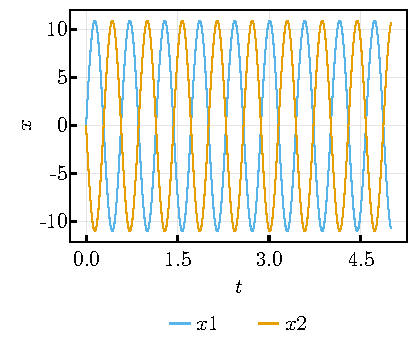
\includegraphics{3spring2mass.pdf}
    \caption{A timeseries view of the three-spring, two-mass system with initial condition $x_1=-1,\dot{x}_1=0, x_2=1,\dot{x}_2=0$.}
    \label{fig: tstm}
\end{figure}

\begin{figure}[ht!]
    \centering
    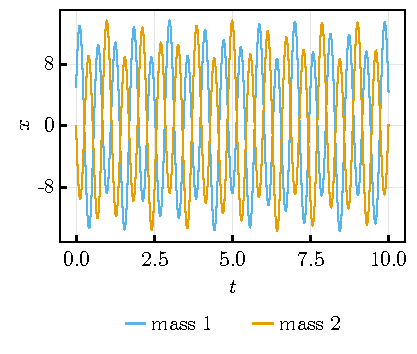
\includegraphics{3spring2mass_with_velocity.pdf}
    \caption{A timeseries view of the three-spring, two-mass system with initial condition $x_1=-1,\dot{x}_1=5, x_2=1,\dot{x}_2=0$.}
    \label{fig: tstm_with_vel}
\end{figure}



\section{The Ray Equation; Fermat's Principle} % q5

The velocity of an object in 2D can be broken down into its basis component, and the line element can be written in terms of velocity.
\[v = \sqrt{x'^2+y'^2}\qquad ds = vdt = \sqrt{x'^2+y'^2}dt\]

Then the total time taken can be calculated by
\[T = \int_P \frac{ds}{c(x,y)} = \int_P \frac{\sqrt{x'^2+y'^2}dt}{c(x,y)} = \int_PF(t,x,x',y,y')dt\]
\[\text{ where }F(t,x,x',y,y') = \frac{\sqrt{x'^2+y'^2}}{c(x,y)}\]

Solving the Euler-Lagrange equation for the curve $x(t)$.
\[\frac{\partial F}{\partial x} = \sqrt{x'^2+y'^2}\frac{\partial}{\partial x}\frac{1}{c(x,y)} = -\frac{\sqrt{x'^2+y'^2}}{c(x,y)^2}\frac{\partial c(x,y)}{\partial x}\]

use the fact that $x' = \frac{dx}{dt}$
\[\frac{d}{d t} \frac{\partial F}{\partial x'} = \frac{d}{dt} \frac{\partial}{\partial x'}\frac{\sqrt{x'^2+y'^2}}{c(x,y)} = \frac{d}{dt} \frac{x'}{c(x,y)\sqrt{x'^2+y'^2}} = \frac{d}{dt} \frac{dx}{c(x,y)\sqrt{x'^2+y'^2}dt}\]

We can convert the independent variable form t to s by multiplying both side of equation 1 by $\frac{dt}{ds} = (x'^2+y'^2)^{\frac{1}{2}}$:
\[\frac{\partial F}{\partial x}\frac{dt}{ds} = -(x'^2+y'^2)^{\frac{1}{2}}\frac{\sqrt{x'^2+y'^2}}{c(x,y)^2}\frac{\partial c(x,y)}{\partial x} = -\frac{1}{c(x,y)^2}\frac{\partial c(x,y)}{\partial x}\]

Using chain rule and the fact that $ds = (x'^2+y'^2)^{\frac{1}{2}} dt$:
\[\frac{d}{d t} \frac{\partial F}{\partial x'} \frac{dt}{ds} = \frac{dt}{ds}\frac{d}{dt} \frac{dx}{c(x,y)\sqrt{x'^2+y'^2}dt} = \frac{d}{ds}\frac{dx}{c(x,y)ds}\].

The exact same procedure can be carry out on the $y(t)$ curve, which together would yield the following system:
\begin{align*}
\frac{d}{ds}\frac{1}{c(x,y)}\frac{dx}{ds} &= -\frac{1}{c(x,y)^2}\frac{\partial c(x,y)}{\partial x}\\
\frac{d}{ds}\frac{1}{c(x,y)}\frac{dy}{ds} &= -\frac{1}{c(x,y)^2}\frac{\partial c(x,y)}{\partial y}
\end{align*}
In fact, the system can be generalized into:

\[\frac{d}{ds} \frac{1}{c(\vec{r})}\frac{d\vec{r}}{ds} = -\frac{1}{c(\vec{r})^2}\nabla c(\vec{r})\]

Where $\vec{r}$ is the position vector of the object and $\nabla$ is the gradient operator, the expression describe a n-equation system component wise.\\
Taking $\vec{r} = (x,y)$ would yield the result derived above.\\

Let's consider ray propagation in a Gradient index (GRIN) medium such as the lens in our eye. Assume the medium is a cylinder shape, the speed of light (i.e. refractive index) varies based on distance from the central optical axis:
\[c = \frac{c_0}{a\sqrt{1-(cr)^2}}\]
where $r$ is radius in cylindrical coordinate, $a$ is the refractive index at the optical axis, $c$ is an arbitrary constant, and $c_0$ is the speed of light in vacuum. Since speed of light is very fast, we will make the assumption that $r << 1$ and thus $ds = dz$.

The parameter of interest is the radial distance from the axis as the ray propagate further into the cylinder, i.e. $r(z)$, the Euler-Lagrange equation then describes:
\begin{align*}
    \frac{d}{dz} \frac{a\sqrt{1-(cr)^2}}{c_0}\frac{d r}{dz} &= -\frac{a^2(1-(cr)^2)}{c_0^2}\frac{\partial}{\partial r} \frac{c_0}{a\sqrt{1-(cr)^2}}\\
    - \frac{ac^2 r}{c_0\sqrt{1-(cr)^2}}\frac{dr}{dz}+\frac{a\sqrt{1-(cr)^2}}{c_0}\frac{d^2 r}{dz^2} &= -\frac{a(1-(cr)^2)}{c_0}\frac{\partial}{\partial r} \frac{1}{\sqrt{1-(cr)^2}}\\
    \sqrt{1-(cr)^2}\frac{d^2 r}{dz^2} &= -(1-(cr)^2)\frac{\partial}{\partial r} \frac{1}{\sqrt{1-(cr)^2}} + \frac{c^2 r}{\sqrt{1-(cr)^2}}\frac{dr}{dz}\\
    \frac{d^2 r}{dz^2} &= -\sqrt{1-(cr)^2} \frac{c^2r}{(1-(cr)^2)^{\frac{3}{2}}}+ \frac{c^2 r}{{1-(cr)^2}}\frac{dr}{dz}\\
    \frac{d^2 r}{dz^2} &= -\frac{c^2r}{(1-(cr)^2)}\left(1-\frac{dr}{dz}\right)\\
\end{align*}

This is a second order autonomous differential equation. The previous approximation can be extended to $\dot{r},cr<<1$, the ODE then reduce to a simple \textit{second order linear homogeneous non-constant coefficient differential equation}, which we know the answer already:
\begin{align*}
    \frac{d^2 r}{dz^2} &= -\frac{c^2r}{(1-(cr)^2)}\left(1-\frac{dr}{dz}\right)\\
    &\approx -c^2 r\\
    \implies r(z) &= A\cos(cz)+B\sin(cz)
\end{align*}
Solving for the initial condition where the light enter at position $\alpha$ with a slope of $\beta$
\begin{align*}
    r(0) &= A\cos(c0)+B\sin(c0) = \alpha \\
    &\implies A = \alpha\\
    r'(0) &= -cA\sin(c0)+cB\cos(c0) = \beta \\
    &\implies B = \frac{\beta}{c}\\
    r(z) &= \alpha\cos(cz)+\frac{\beta}{c}\sin(cz)
\end{align*}

The ray oscillates back and forth across the optical axis, as shown in \Fref{fig: rays}, where the light enters the cylinder at $z=0$, and a lighter color indicating a faster speed of light. Both light, despite entering at different $r$ value, meet at the same $z$ when they reach $r = 0$. This property allows the GRIN medium to be a great candidate as a lens. In fact this is how human eyes, which is a GRIN material, focus the light for further object, as the light entering is essentially perpendicular to our eyes, the eye muscle shapes the lens into cylindrical shape to focus light into our receptor.

\begin{figure}
    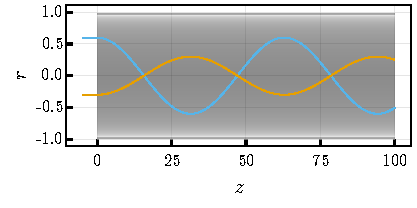
\includegraphics{rays.pdf}
    \caption{Two rays of light enter into the nonlinear medium, and exhibit sinusoidal oscillations.}
    \label{fig: rays}
\end{figure}

\begin{figure}
    \begin{subfigure}{.5\textwidth}
      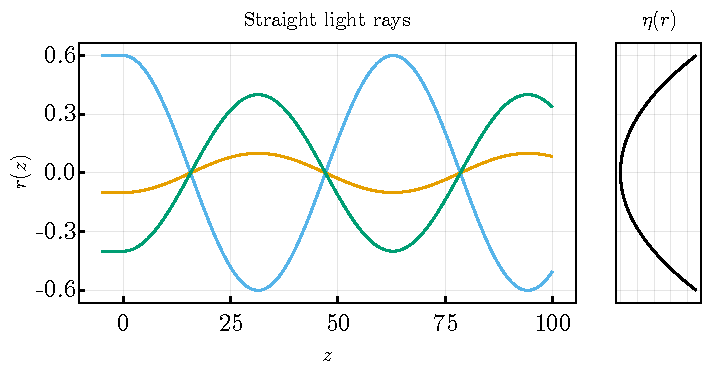
\includegraphics[width=.9\linewidth]{ray_sim.pdf}
      \caption{Light Entering straight}
    \end{subfigure}%
    \begin{subfigure}{.5\textwidth}
      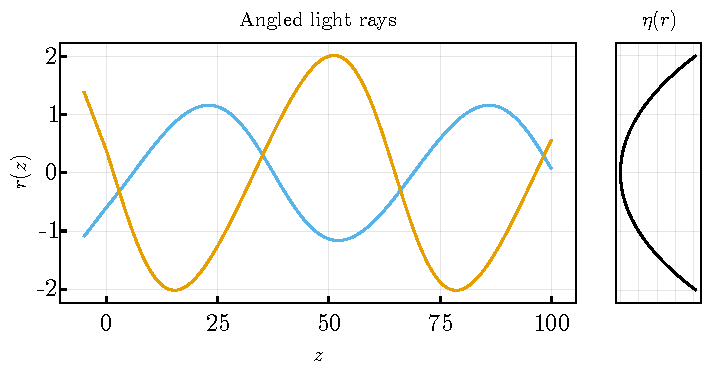
\includegraphics[width=.9\linewidth]{ray_sim_angled.pdf}
      \caption{Light Entering in an angle}
    \end{subfigure}
    \caption{Sample trajectories (numerically solved) of light rays in our nonlinear medium.}
    \label{fig: comp}
\end{figure}

\begin{figure}
    \begin{subfigure}{.5\textwidth}
      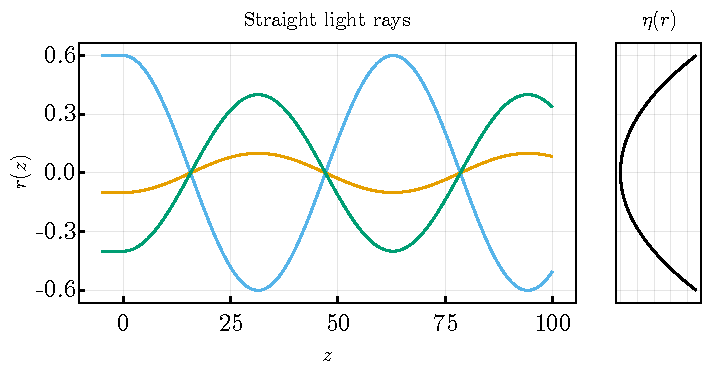
\includegraphics[width=.9\linewidth]{ray_comp.pdf}
      \caption{Light entering normal to the medium.}
    \end{subfigure}%
    \begin{subfigure}{.5\textwidth}
      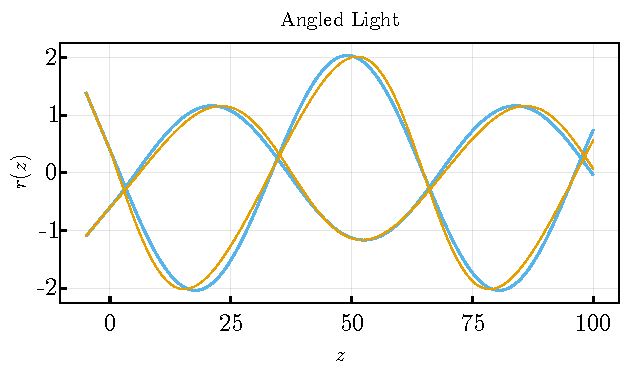
\includegraphics[width=.9\linewidth]{ray_comp_angled.pdf}
      \caption{Light entering in at an angle to the medium.}
    \end{subfigure}
    \caption{Comparison between approximated solution and numerical solution to the original ODE.  Blue lines represent the approximation, whereas orange lines represent the numerical solution.}
    \label{fig: anal_sim}
\end{figure}



\Fref{fig: anal_sim} shows a comparison between the approximated result (in Blue) and the solution to the original equation by numerical method (in Orange), again the light enters the cylinder at $z=0$. The two line very closely overlap for light entering straight and in an angle, hence a valid approximation for $cr << 1$.

\section{Conclusion}

The advantage of the Euler-Lagrange equations are that they work for any coordinate system (not just the Cartesian system), and are much more general than the Newtonian $F = ma$. They also have an interesting application, called the geodesic. A geodesic curve allows us to find the shortest path between two points on a curved surface, or a “straight line" with respect to the surface. Solving these geodesic equations proves to be particularly useful in general relativity, where the geodesic represents the shortest path between two points in a curved space-time. The Euler-Lagrange equations are powerful tools to solve messy, physical systems.

\end{document}
